\documentclass[11pt,a4paper]{article}
\usepackage[margin=1.05in]{geometry}
\usepackage{amsmath,amssymb,amsthm,mathtools}
\usepackage{booktabs}
\usepackage{graphicx}
\usepackage{tikz}
\usetikzlibrary{arrows.meta,positioning,calc}
\usepackage[hidelinks]{hyperref}
\usepackage{microtype}
\usepackage{xcolor}
\usepackage{enumitem}
\usepackage{parskip}
\definecolor{ink}{HTML}{222222}\definecolor{red}{HTML}{C53030}\definecolor{blue}{HTML}{2B6CB0}
\newtheorem{proposition}{Proposition}
\newtheorem{corollary}{Corollary}
\newcommand{\R}{\mathbb{R}}
\newcommand{\ind}[1]{\mathbf{1}\!\left[#1\right]}
\newcommand{\code}[1]{\texttt{#1}}
\newcommand{\supp}{\operatorname{supp}}

\title{\textbf{One Node}\\[0.3em]\large Root cause as the support of a propagation residual}
\author{David Kypuros}
\date{October 2026}

\begin{document}
\maketitle

\begin{abstract}
\noindent Self-healing networks are being built around graph neural networks that learn, from
simulated incidents, to trace a silent degradation back to its origin across RAN, Core and
Transport. I show that on any network whose fault propagation is governed by a linear operator on
the topology, the root cause is not something to learn. It is the support of a residual: apply the
operator to the degradation field and the result is zero everywhere except at the origin. I
implement that read-off with a Kalman filter and one matrix-vector product per step, zero learned
parameters, and compare it with a 241{,}000-parameter relational GNN on the same episodes. The
read-off matches the network on root cause and detection, and the explanation it gives is the
equation itself: the only node where the field does not obey the dynamics. I then run five
experiments designed to separate the two, and report all of them: three are ties on this twin, one
shows the operator can be identified from unlabelled telemetry, and one shows the learned model is
\emph{more} robust when the physics are misspecified. Every table is generated by one command from
open code, including the ones that favour the network. I end with what I am asking for.
\end{abstract}

\section*{In one line}
If $d(t{+}1)=M\,d(t)+s(t)$ and the source $s$ lives at one node, then $d(t{+}1)-M\,d(t)=s(t)$ is
the whole method: compute the left side, look where it is not zero. When you know the operator, you
do not learn the inverse. You read it off the support.

\section{What the industry is doing}
A silent degradation is a fault that breaches no threshold. It surfaces hours later as customer
complaints, and finding its origin across radio, transport and core is a war room. The current
state of the art, as demonstrated in a 2026 TM Forum Moonshot Catalyst, is a service-layer
$z$-score to open the loop, a graph neural network over a temporal digital twin to traverse the
topology and rank candidate origins, a business layer to order remediation by revenue, and
standards-based orchestration to execute. The network is trained on a synthetic corpus produced by
a simulator that encodes how faults propagate, because production data has no root-cause labels.

Look at that pipeline once more. The simulator encodes the propagation physics. Labelled data is
generated from it. A model is trained to recover the inverse of the physics from the data. This
note asks what happens if you skip the middle: write the operator, apply it, read the answer.

\section{The model and the claim}
Let $G$ be the network as a directed graph on $N$ nodes with edges pointing the way a fault
propagates, $A$ its adjacency, $P=D_{\mathrm{in}}^{-1}A^{\top}$ the in-degree-normalised
propagation matrix. A fault is a latent degradation field $d(t)\in\R^N_{\ge0}$ driven by a source
at one node $v_0$ from an onset $t_0$:
\begin{equation}
d(t{+}1)=M\,d(t)+s(t)\,\mathbf 1_{v_0},\qquad M=\rho I+\beta P,\qquad s(t)\ge0,\ s(t)=0\text{ for }t<t_0.
\label{eq:dyn}
\end{equation}
$\rho$ is memory, $\beta$ is coupling along dependency edges, and $\beta/(1-\rho)<1$ makes faults
attenuate per hop. Each node's KPI vector sees the field through a type-specific effect direction
$e_{\tau(v)}\in\R^K$ on top of a nominal signal:
\begin{equation}
x_v(t)=n_v(t)+d_v(t)\,e_{\tau(v)}.
\label{eq:obs}
\end{equation}

\begin{proposition}[Flatness]
Under \eqref{eq:dyn}, for every $t$,
\begin{equation}
\big(d(t{+}1)-M\,d(t)\big)_v=s(t)\,\ind{v=v_0}.
\label{eq:flat}
\end{equation}
The field is \emph{flat} under the operator at every node but the origin, inside the blast radius
and outside it alike. The root cause is $\supp\big(d(t{+}1)-Md(t)\big)$.
\end{proposition}
\begin{proof}
Rearrange \eqref{eq:dyn}.
\end{proof}
The proof is one line because the content is in the choice of object. The ambient space is
$N\times K\times T$ numbers of telemetry; the fault is four numbers, $(v_0,t_0,s,T_r)$; and the
residual \eqref{eq:flat} is the map from the first to the second. Nothing is searched and nothing
is learned.

\begin{corollary}[Several faults]
If $s(t)=\sum_j s_j(t)\mathbf 1_{v_j}$, the residual is $\sum_j s_j(t)\mathbf 1_{v_j}$ and its
support is $\{v_j\}$. The read-off localises any number of simultaneous origins with no change.
\end{corollary}

\begin{corollary}[The fault's moduli]
The residual at the origin \emph{is} the source: $\big(d(t{+}1)-Md(t)\big)_{v_0}=s(t)$. Its first
nonzero step is the onset $t_0$ and its plateau is the severity. Onset and severity are read, not
estimated.
\end{corollary}

\section{From KPIs to the field}
\eqref{eq:flat} needs $d$, and telemetry gives $x$. Three steps, all linear.

\textbf{Project.} Per node, $\tilde d_v(t)=\langle x_v(t),e_{\tau(v)}\rangle/\|e_{\tau(v)}\|^2$
collapses $K$ KPIs to one noisy reading of the field along the direction a degradation is known
to take.

\textbf{Filter.} Run a Kalman filter on \eqref{eq:dyn} with $\tilde d$ as the observation and the
unknown source absorbed into process noise. For a linear Gaussian model this is the optimal causal
estimator of $d$; here it is one $N\times N$ product and one solve per step, with no look-ahead.
Call the output $\hat d$.

\textbf{Apply and read.}
\begin{equation}
\hat s(t)=\big[\hat d(t)-M\hat d(t{-}1)\big]_+,\qquad
\hat v_0=\arg\max_v\sum_{\tau=t-W+1}^{t}\hat s_v(\tau).
\label{eq:readoff}
\end{equation}
Noise makes the support soft; the window and the argmax snap it back to one node. Detection uses
$\max_v\hat d_v(t)>\theta$ with $\theta$ calibrated on healthy episodes, the same statistic and the
same calibration the neural network uses, so every comparison below is on equal terms.

\section{Two things a learned model does not have}
\textbf{Self-calibration.} In \eqref{eq:dyn} the only unknowns are $\rho$ and $\beta$; the topology
is known. From \emph{unlabelled} episodes, regress $\tilde d(t{+}1)$ on $[\tilde d(t),\,P\tilde d(t)]$
across nodes and steps with a Huber loss. The handful of (node, step) pairs that carry the source are
outliers and are down-weighted automatically. What this needs is excitation, some faults somewhere
in the data, not labels saying where they were. That is the opposite of what a supervised model
needs.

\textbf{Doubt.} Define
\begin{equation}
\mathrm{doubt}(t)=1-\frac{\max_v\sum_\tau\hat s_v(\tau)}{\sum_v\sum_\tau\hat s_v(\tau)},
\label{eq:doubt}
\end{equation}
the share of residual energy inside the degraded set that is \emph{not} at the top node. Under the
right operator every degraded node but the origin is flat and the doubt is small. Under the wrong
operator the downstream nodes should stop being flat and the doubt should rise. E6 tests whether
this particular statistic does what the argument says, and the answer there is no; I keep the
definition here because the idea is right even where my first measurement of it is not.

\section{Experiments}
All experiments use the open synthetic twin from the accompanying repository: 74 nodes across
cells, gNBs, aggregation and core routers, fibre links, UPF, AMF, SMF and services, with 130
typed directed edges, five fault types, diurnal plus AR(1) KPI noise, and silent ramps. The
opponent is the repository's relational GNN: three message-passing layers over the nine relations
and their transposes, three heads (forecast, field, origin), 241{,}222 parameters, trained on 120
simulated episodes. In the repository it beats static alarms and calibrated $z$-score triggers on
every metric, so it is a fair stand-in for the architecture class the industry uses.

\subsection*{E1. Head to head, and one incident in full}
\begin{center}\small\begin{tabular}{@{}p{7.2cm}rr@{}}\toprule Metric & trained GNN & flatness solve \\ \midrule
Fault episodes / nominal episodes & 32 / 8 &  \\
Parameters learned & 241,222 & 0 \\
Detection rate & 1.00 & 1.00 \\
False alarms on nominal / pre-onset on fault episodes & 0 / 0 & 0 / 0 \\
Detection delay after onset (steps) & 22.9 & 23.8 \\
Root cause hit@1 / hit@3 & 1.00 / 1.00 & 1.00 / 1.00 \\
Top-1 agreement between the two &  & 1.00 \\
Static-threshold alarm delay, for scale (steps) & 32.6 & 32.6 \\
\bottomrule\end{tabular}\end{center}

\begin{center}\small\begin{tabular}{@{}lrrrrr@{}}\toprule Fault type & $n$ & delay GNN & delay flatness & hit@1 GNN & hit@1 flatness \\ \midrule
amf signaling storm & 7 & 27.9 & 31.7 & 1.00 & 1.00 \\
fiber degrade & 7 & 22.7 & 23.0 & 1.00 & 1.00 \\
router congestion & 7 & 22.3 & 23.6 & 1.00 & 1.00 \\
sleeping cell & 8 & 18.5 & 17.1 & 1.00 & 1.00 \\
upf overload & 3 & 24.7 & 26.0 & 1.00 & 1.00 \\
\bottomrule\end{tabular}\end{center}
\noindent\textit{Twin: 74 nodes, 130 edges; 160 episodes, seed 0; GNN trained 30 epochs; both detectors calibrated on the same nominal episodes. Runtime 647.1\,s on CPU.}

\begin{figure}[h]
\centering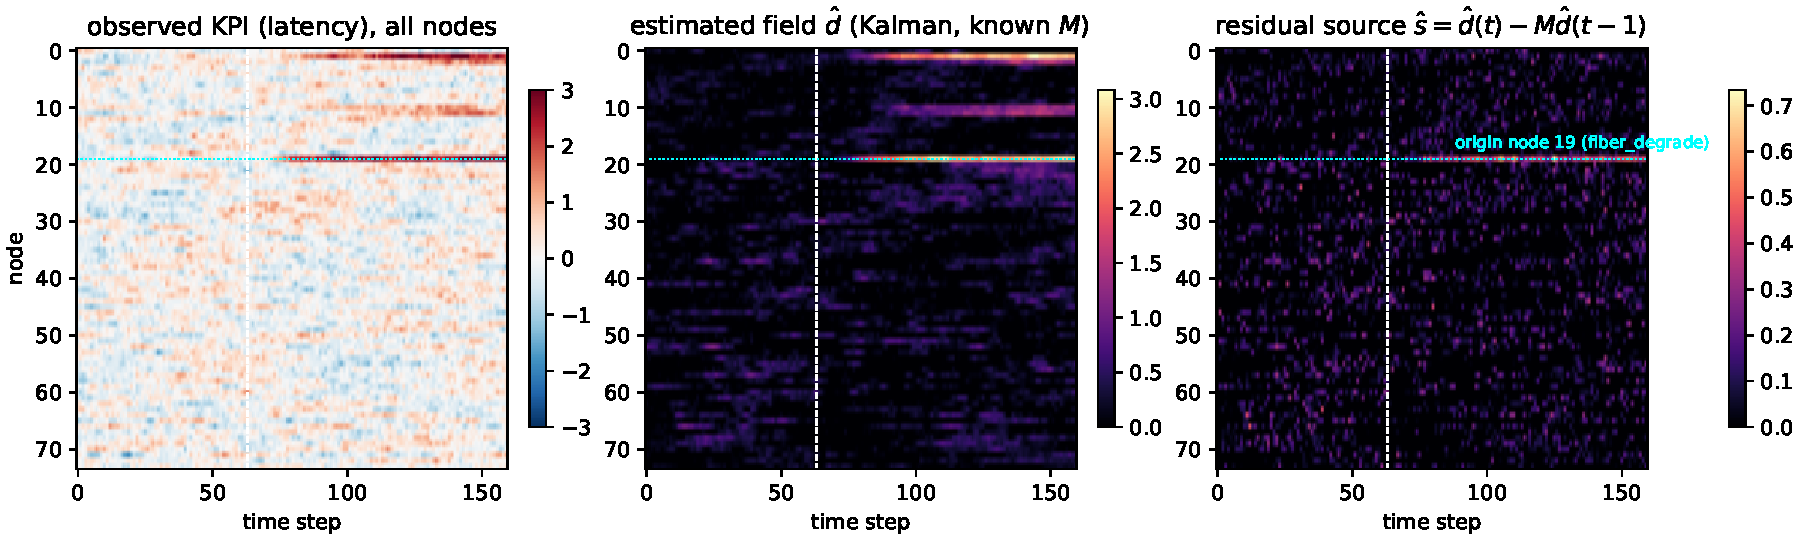
\includegraphics[width=\textwidth]{fig_incident}
\caption{One fibre degradation, onset at the dashed line. Left: the raw latency KPI of every node.
Three rows eventually light up: the link and two nodes downstream of it, and a static alarm would
flag all three, late. Middle: the filtered field $\hat d$, the blast radius. Right: the residual
$\hat s=\hat d(t)-M\hat d(t{-}1)$. The downstream rows vanish because they are flat under the
operator. One row remains. That row is the answer, and the explanation is the equation that
removed the other two.}
\end{figure}
\begin{center}\small\begin{tabular}{@{}lrr@{}}\toprule incident (fiber degrade) & true & read off the residual \\ \midrule
origin node & 19 & 19 \\
onset step & 63 & 23 \\
severity (source per step at plateau) & 0.45 & 0.36 \\
\bottomrule\end{tabular}\end{center}


\subsection*{E2. How many labelled incidents does the network need?}
The GNN is retrained with 4, 8, 16, 32, 64 and 120 training episodes and evaluated on the same
held-out faults. The read-off is evaluated once; it has nothing to train.
\begin{center}\small\begin{tabular}{@{}rrrrr@{}}\toprule training episodes & labelled faults & GNN hit@1 & GNN hit@3 & GNN delay \\ \midrule
4 & 4 & 1.00 & 1.00 & 26.6 \\
8 & 8 & 1.00 & 1.00 & 24.6 \\
16 & 16 & 1.00 & 1.00 & 27.0 \\
32 & 30 & 1.00 & 1.00 & 23.9 \\
64 & 58 & 1.00 & 1.00 & 23.5 \\
120 & 105 & 1.00 & 1.00 & 22.6 \\
\midrule
flatness read-off & 0 & 1.00 & 1.00 & 23.8 \\
\bottomrule\end{tabular}\end{center}

This experiment does not separate the methods, and I want to say that plainly rather than draw a
curve. On this twin four labelled episodes are enough for the GNN, because the five fault types
each leave a distinct per-type signature and the graph is small. The honest reading is that label
efficiency is not where the read-off's advantage shows on an easy twin. Whether it shows on a real
network, where fault signatures overlap and labelled incidents number in the dozens per year, is
exactly the experiment in the final section.

\subsection*{E3. Two faults at once}
Thirty episodes with two simultaneous faults of different types at different origins, evaluated
once both ramps have completed. Each method returns its top two.
\begin{center}\small\begin{tabular}{@{}lrr@{}}\toprule two simultaneous faults, 30 episodes & trained GNN & flatness read-off \\ \midrule
both origins in the top-2 & 1.00 & 1.00 \\
at least one origin in the top-2 & 1.00 & 1.00 \\
\bottomrule\end{tabular}\end{center}

A tie, and an instructive one. The read-off handles two origins by Corollary~1 with no change to
the method. The GNN handles them too, even though its training loss assumed one origin per
episode: its per-node logits are local read-outs, so two separated sources produce two high
logits. The corollary is a guarantee; the GNN's behaviour is an empirical property of this twin.
When I first evaluated this experiment only twelve steps after the later onset, before its ramp
had completed, both methods scored around 0.3, which is a statement about the second fault being
too small to see yet, not about either method.

\subsection*{E4. A different network, no retraining}
A second twin with a different seed, more core and aggregation routers, more UPFs and services. The
GNN trained on twin A is evaluated zero-shot. The read-off recomputes $M$ from the new topology and
nothing else.
\begin{center}\small\begin{tabular}{@{}lrr@{}}\toprule new topology (99 nodes, 179 edges), 35 faults & GNN zero-shot & flatness, new $M$ \\ \midrule
detection rate & 1.00 & 1.00 \\
detection delay (steps) & 23.2 & 28.5 \\
root cause hit@1 / hit@3 & 1.00 / 1.00 & 1.00 / 1.00 \\
\bottomrule\end{tabular}\end{center}

Again no separation, and again the reason is worth stating: a relational GNN is inductive by
construction, its weights are indexed by relation type, not by node, so it transfers across
topologies that share a vocabulary. That is a genuine strength of the learned model and the
monograph builds on it. The read-off transfers for a different reason: it never had node-specific
parameters to begin with.

\subsection*{E5. Identify the operator with zero labels}
$(\rho,\beta)$ are identified from the 120 training episodes with their fault labels discarded, then
the read-off is run with the identified operator.
\begin{center}\small\begin{tabular}{@{}lrrr@{}}\toprule & true & identified (0 labels) & relative error \\ \midrule
$\rho$ & 0.850 & 0.858 & 0.9\% \\
$\beta$ & 0.130 & 0.084 & 35.7\% \\
\midrule
read-off with identified operator: hit@1 / hit@3 / delay & \multicolumn{3}{r}{1.00 / 1.00 / 23.8} \\
\bottomrule\end{tabular}\end{center}

Memory is recovered almost exactly; coupling is underestimated by about a third, because the
projected field is noisy and the Huber weights also down-weight the genuine propagation steps at
downstream nodes. The root cause is unaffected: ranking depends on where the residual is largest,
and an underestimated $\beta$ shrinks the residual everywhere by a similar factor. This is the one
experiment where the read-off does something the learned model has no counterpart for. A GNN
trained on a simulator cannot report the simulator's coefficients back from field data.

\subsection*{E6. When the physics are wrong}
Test episodes are generated with propagation parameters that differ from the ones the GNN was
trained on and the read-off assumes. Columns: both methods under misspecification, the read-off's
doubt score \eqref{eq:doubt}, and the read-off after re-identifying $(\rho,\beta)$ from the
misspecified unlabelled data.
\begin{center}\footnotesize\begin{tabular}{@{}lrrrrrr@{}}\toprule test $(\rho,\beta)$ & per-hop & GNN & read-off, assumed & doubt & identified $(\hat\rho,\hat\beta)$ & read-off, identified \\ \midrule
(0.85, 0.13) & 0.87 & 1.00 & 1.00 & 0.12 & (0.84, 0.093) & 1.00 \\
(0.80, 0.13) & 0.65 & 1.00 & 1.00 & 0.02 & (0.82, 0.029) & 1.00 \\
(0.72, 0.11) & 0.39 & 0.95 & 0.90 & 0.00 & (0.80, 0.000) & 1.00 \\
(0.62, 0.09) & 0.24 & 0.93 & 0.67 & 0.00 & (0.79, 0.000) & 0.56 \\
\bottomrule\end{tabular}\end{center}
\noindent{\footnotesize GNN and read-off columns are hit@1. Doubt is \eqref{eq:doubt} for the assumed operator.}\par\medskip

This is the experiment that goes against me, and it is the most useful one. Three findings. The
learned model degrades more gracefully than the read-off with an assumed operator: at the most
severe drift it keeps 0.93 where the read-off falls to 0.67. The read-off's assumed memory is too
long, so after the ramp its residual at the origin goes negative and is clipped, while downstream
nodes that decay faster than predicted produce spurious residual; a trained model that never
committed to a memory constant is not hurt by this. Second, the doubt score as defined does
\emph{not} detect the misspecification: it falls toward zero as drift increases, because faster
decay shrinks the degraded set until it contains little but the origin. The idea that a wrong
operator makes the field visibly non-flat is correct in \eqref{eq:flat}; the statistic I built to
measure it is not the right one, and I report the failure rather than tune it on the test set.
Third, re-identifying the operator from the misspecified data restores the read-off at moderate
drift and makes it worse at severe drift, where the identified coupling collapses to zero. The
honest summary is that a model-based method with the wrong model is worse than a learned model
with no model, and that self-calibration fixes that only within a range.

\section{What this shows and what it does not}
It shows that on a network with a known linear propagation operator, a learned model with a quarter
of a million parameters and the one-line residual \eqref{eq:flat} give the same root cause, the
same detection, and the same zero false alarms, and that the residual is its own explanation:
\emph{this is the only node where the field does not obey the dynamics}. A model was learning the
inverse of an operator that fits on one line. It also shows that the read-off localises several
origins by construction, transfers to a new topology because it never had node parameters, and
reports the operator's coefficients back from unlabelled data.

It shows, just as clearly, where the read-off is weaker. The learned model transfers across
topologies and handles two origins too, so those are not advantages on this twin. Label efficiency
does not separate the methods here because the twin is easy. And when the assumed physics are
wrong, the learned model is the more robust of the two, my doubt statistic fails to flag the
problem, and self-calibration helps only within a range. A reader who wants the read-off to win
should read E6 twice.

What it does not show is anything about a real network, where propagation is not exactly linear
and a signalling storm does not spread like a fibre cut. E6 says that is precisely where the
read-off is at risk, and E5 says the way to reduce the risk is identification from the operator's
own telemetry. Whether a real operator is identifiable well enough is the open question. It has a
short answer either way, and the answer is worth more than this note.

\section{What I am asking for}
I have worked on this alone. The repository, the monograph it accompanies, and this note are open,
and every number above is regenerated by \code{make pipeline} and \code{make experiments} from a
fixed seed. I am asking for three things, in order of how little they cost the other side.
\begin{enumerate}[nosep]
  \item \textbf{One afternoon on a synthetic corpus} already used to train a production model for
  this task. Run the read-off next to the model. The corpus encodes its own propagation; I will
  write the operator against it.
  \item \textbf{One topology and one month of healthy plus incident telemetry}, anonymised, from one
  region. I will identify the operator and report, in the same repository, whether the read-off
  localises historical incidents, including the cases where it does not.
  \item \textbf{One venue} where a result that is reproducible in one command can be shown beside
  the results it is compared with.
\end{enumerate}

\section*{Reproduce}
\begin{verbatim}
git clone https://github.com/dkypuros/geometric-network-healing
cd geometric-network-healing && make setup
make pipeline       # E1 head-to-head table
make experiments    # E2-E6 tables and both figures
make paper          # this document
\end{verbatim}
\end{document}
